%\section*{Pregunta 4b}
\Large

b) El Problema de las Ocho Reinas consiste en acomodar ocho reinas de ajedrez en un tablero, sin que ninguna de éstas se ataque entre sí. Una reina, puede atacar (a) de forma vertical, (b) de forma horizontal y (c) en diagonal. Usando estas reglas, indicar si el siguiente tablero es una solución al problema de las ocho reinas.\\

\begin{figure}[h!]
\centering
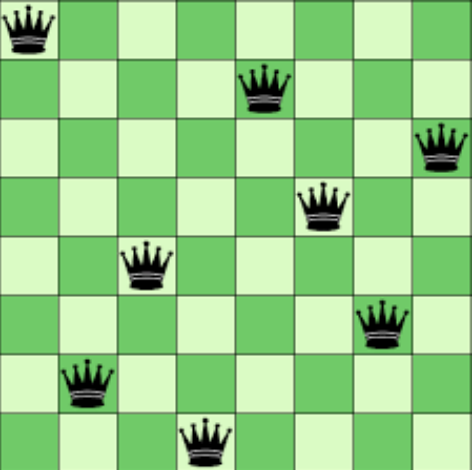
\includegraphics[scale=0.35]{Tablero.png}
\end{figure}
\large

Este problema tiene varias formas de solucionarse, sin embargo la más efectiva que encontramos, es por medio del backtracking,
sin embargo, el backtracking es mucho más efectivo con lenguajes de programación declarativos, ya sean lógicos o funcionales,
pues como se mencionó en clase, no hay recursión más pura que la de un lenguaje de programación declarativo.
